70. \begin{figure}[ht!]
\center{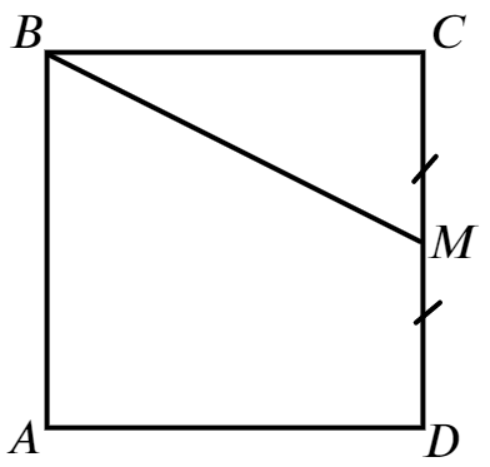
\includegraphics[scale=0.35]{g8-70.png}}
\end{figure}\\
Пусть сторона квадрата равна $a,$ тогда по теореме Пифагора для треугольника $BMC$ имеем $3^2=a^2+\cfrac{1}{4}a^2,\ a^2=\cfrac{36}{5}\text{ см}^2,$ а $S=a^2=\cfrac{36}{5}\text{ см}^2.$
ewpage
oindent
